%% LyX 2.2.1 created this file.  For more info, see http://www.lyx.org/.
%% Do not edit unless you really know what you are doing.
\documentclass[english]{article}
\usepackage[T1]{fontenc}
\usepackage{geometry}
\geometry{verbose}
\usepackage{array}
\usepackage{multirow}
\usepackage{amsmath}
\usepackage{graphicx}

\makeatletter

%%%%%%%%%%%%%%%%%%%%%%%%%%%%%% LyX specific LaTeX commands.
%% Because html converters don't know tabularnewline
\providecommand{\tabularnewline}{\\}

%%%%%%%%%%%%%%%%%%%%%%%%%%%%%% User specified LaTeX commands.
\usepackage{inputenc}
\usepackage{authblk}
\usepackage{url}
\usepackage{ulem}
\author[1,2,4]{Daniel Schlauch} 
\author[1,3]{Heide Fier}
\author[1,4]{Christoph Lange}
\affil[1]{Department of Biostatistics, Harvard TH Chan School of Public Health, Boston, MA 02115}
\affil[2]{Department of Biostatistics and Computational Biology, Dana-Farber Cancer Institute, Boston, MA 02115}
\affil[3]{Institute of Genomic Mathematics, University of Bonn, Bonn, Germany}
\affil[4]{Channing Division of Network Medicine,  Brigham and Women's Hospital, 181 Longwood Ave; CL-3; Boston, MA 02115}

\makeatother

\usepackage{babel}
\begin{document}

\title{\textbf{Supplementary Materials for} \\
Identification of genetic outliers due to sub-structure and cryptic
relationships}

\maketitle
\renewcommand{\figurename}{Supplemental Figure}
\renewcommand{\tablename}{Supplemental Table}

\section{Supplementary Materials}

\subsection{Example of $\hat{s}_{i,j}$ computation}

Consider a binary matrix of 20 haploid genomes from 10 samples (labeled
a-t).

The matrix $\boldsymbol{G}$ is encoded such that 1 indicates the
presence of the minor allele and 0 indicates the presence of the major
allele for a particular variant (column) and haploid sample (row).
For visual purposes, we limit the calculation to 4 variants and we
show $\boldsymbol{G}^{T}$ here:

\begin{tabular}{|c||c|c|c|c|c|c|c|c|c|c|c|c|c|c|c|c|c|c|c|c|}
\cline{2-21} 
\multicolumn{1}{c|}{} & a & b & c & d & e & f & g & h & i & j & k & l & m & n & o & p & q & r & s & t\tabularnewline
\hline 
variant 1 & 0 & 0 & 0 & 0 & 0 & 0 & 1 & 0 & 0 & 0 & 0 & 0 & 0 & 1 & 0 & 0 & 0 & 0 & 0 & 0\tabularnewline
\hline 
variant 2 & 1 & 0 & 1 & 0 & 1 & 0 & 1 & 0 & 1 & 0 & 1 & 0 & 1 & 0 & 1 & 0 & 1 & 0 & 1 & 0\tabularnewline
\hline 
variant 3 & 1 & 1 & 1 & 1 & 1 & 1 & 1 & 1 & 1 & 1 & 0 & 0 & 0 & 0 & 0 & 0 & 0 & 0 & 0 & 0\tabularnewline
\hline 
variant 4 & 0 & 0 & 0 & 0 & 0 & 0 & 0 & 0 & 0 & 0 & 1 & 1 & 1 & 1 & 1 & 1 & 1 & 1 & 1 & 1\tabularnewline
\hline 
\end{tabular}

For the purposes of this explanatory example, note that columns g
and n share the low frequency allele (1), but differ along the common
variants (2-4). Intuitively, we want to consider the relative informativeness
of the low frequency variant compared to the common variants.

The minor allele frequencies for variants 1,2,3,4 are 0.1, 0.5, 0.5,
and 0.5, respectively. 

For each locus, we compute $w_{k}$, $k\in\left\{ 1,2,3,4\right\} $
\[
w_{k}=\frac{{20 \choose 2}}{{\sum_{l=1}^{20}\boldsymbol{G}_{l,k} \choose 2}}
\]
Such that $w_{1}=190$ and $w_{2}=w_{3}=w_{4}=4.22$

Using equation (1), we compute the relatedness matrix for across these
variants:

 \resizebox{\columnwidth}{!}{%

\begin{tabular}{c|c|c|c|c|c|c|c|c|c|c|c|c|c|c|c|c|c|c|c|c|}
\multicolumn{1}{c}{} & \multicolumn{1}{c}{a} & \multicolumn{1}{c}{b} & \multicolumn{1}{c}{c} & \multicolumn{1}{c}{d} & \multicolumn{1}{c}{e} & \multicolumn{1}{c}{f} & \multicolumn{1}{c}{g} & \multicolumn{1}{c}{h} & \multicolumn{1}{c}{i} & \multicolumn{1}{c}{j} & \multicolumn{1}{c}{k} & \multicolumn{1}{c}{l} & \multicolumn{1}{c}{m} & \multicolumn{1}{c}{n} & \multicolumn{1}{c}{o} & \multicolumn{1}{c}{p} & \multicolumn{1}{c}{q} & \multicolumn{1}{c}{r} & \multicolumn{1}{c}{s} & \multicolumn{1}{c}{t}\tabularnewline
\cline{2-21} 
a & - & 4.2 & 8.4 & 4.2 & 8.4 & 4.2 & 8.4 & 4.2 & 8.4 & 4.2 & 4.2 & 0 & 4.2 & 0 & 4.2 & 0 & 4.2 & 0 & 4.2 & 0\tabularnewline
\cline{2-21} 
b & 4.2 & - & 4.2 & 4.2 & 4.2 & 4.2 & 4.2 & 4.2 & 4.2 & 4.2 & 0 & 0 & 0 & 0 & 0 & 0 & 0 & 0 & 0 & 0\tabularnewline
\cline{2-21} 
c & 8.4 & 4.2 & - & 4.2 & 8.4 & 4.2 & 8.4 & 4.2 & 8.4 & 4.2 & 4.2 & 0 & 4.2 & 0 & 4.2 & 0 & 4.2 & 0 & 4.2 & 0\tabularnewline
\cline{2-21} 
d & 4.2 & 4.2 & 4.2 & - & 4.2 & 4.2 & 4.2 & 4.2 & 4.2 & 4.2 & 0 & 0 & 0 & 0 & 0 & 0 & 0 & 0 & 0 & 0\tabularnewline
\cline{2-21} 
e & 8.4 & 4.2 & 8.4 & 4.2 & - & 4.2 & 8.4 & 4.2 & 8.4 & 4.2 & 4.2 & 0 & 4.2 & 0 & 4.2 & 0 & 4.2 & 0 & 4.2 & 0\tabularnewline
\cline{2-21} 
f & 4.2 & 4.2 & 4.2 & 4.2 & 4.2 & - & 4.2 & 4.2 & 4.2 & 4.2 & 0 & 0 & 0 & 0 & 0 & 0 & 0 & 0 & 0 & 0\tabularnewline
\cline{2-21} 
g & 8.4 & 4.2 & 8.4 & 4.2 & 8.4 & 4.2 & - & 4.2 & 8.4 & 4.2 & 4.2 & 0 & 4.2 & \textbf{190} & 4.2 & 0 & 4.2 & 0 & 4.2 & 0\tabularnewline
\cline{2-21} 
h & 4.2 & 4.2 & 4.2 & 4.2 & 4.2 & 4.2 & 4.2 & - & 4.2 & 4.2 & 0 & 0 & 0 & 0 & 0 & 0 & 0 & 0 & 0 & 0\tabularnewline
\cline{2-21} 
i & 8.4 & 4.2 & 8.4 & 4.2 & 8.4 & 4.2 & 8.4 & 4.2 & - & 4.2 & 4.2 & 0 & 4.2 & 0 & 4.2 & 0 & 4.2 & 0 & 4.2 & 0\tabularnewline
\cline{2-21} 
j & 4.2 & 4.2 & 4.2 & 4.2 & 4.2 & 4.2 & 4.2 & 4.2 & 4.2 & - & 0 & 0 & 0 & 0 & 0 & 0 & 0 & 0 & 0 & 0\tabularnewline
\cline{2-21} 
k & 4.2 & 0 & 4.2 & 0 & 4.2 & 0 & 4.2 & 0 & 4.2 & 0 & - & 4.2 & 8.4 & 4.2 & 8.4 & 4.2 & 8.4 & 4.2 & 8.4 & 4.2\tabularnewline
\cline{2-21} 
l & 0 & 0 & 0 & 0 & 0 & 0 & 0 & 0 & 0 & 0 & 4.2 & - & 4.2 & 4.2 & 4.2 & 4.2 & 4.2 & 4.2 & 4.2 & 4.2\tabularnewline
\cline{2-21} 
m & 4.2 & 0 & 4.2 & 0 & 4.2 & 0 & 4.2 & 0 & 4.2 & 0 & 8.4 & 4.2 & - & 4.2 & 8.4 & 4.2 & 8.4 & 4.2 & 8.4 & 4.2\tabularnewline
\cline{2-21} 
n & 0 & 0 & 0 & 0 & 0 & 0 & \textbf{190} & 0 & 0 & 0 & 4.2 & 4.2 & 4.2 & - & 4.2 & 4.2 & 4.2 & 4.2 & 4.2 & 4.2\tabularnewline
\cline{2-21} 
o & 4.2 & 0 & 4.2 & 0 & 4.2 & 0 & 4.2 & 0 & 4.2 & 0 & 8.4 & 4.2 & 8.4 & 4.2 & - & 4.2 & 8.4 & 4.2 & 8.4 & 4.2\tabularnewline
\cline{2-21} 
p & 0 & 0 & 0 & 0 & 0 & 0 & 0 & 0 & 0 & 0 & 4.2 & 4.2 & 4.2 & 4.2 & 4.2 & - & 4.2 & 4.2 & 4.2 & 4.2\tabularnewline
\cline{2-21} 
q & 4.2 & 0 & 4.2 & 0 & 4.2 & 0 & 4.2 & 0 & 4.2 & 0 & 8.4 & 4.2 & 8.4 & 4.2 & 8.4 & 4.2 & - & 4.2 & 8.4 & 4.2\tabularnewline
\cline{2-21} 
r & 0 & 0 & 0 & 0 & 0 & 0 & 0 & 0 & 0 & 0 & 4.2 & 4.2 & 4.2 & 4.2 & 4.2 & 4.2 & 4.2 & - & 4.2 & 4.2\tabularnewline
\cline{2-21} 
s & 4.2 & 0 & 4.2 & 0 & 4.2 & 0 & 4.2 & 0 & 4.2 & 0 & 8.4 & 4.2 & 8.4 & 4.2 & 8.4 & 4.2 & 8.4 & 4.2 & - & 4.2\tabularnewline
\cline{2-21} 
t & 0 & 0 & 0 & 0 & 0 & 0 & 0 & 0 & 0 & 0 & 4.2 & 4.2 & 4.2 & 4.2 & 4.2 & 4.2 & 4.2 & 4.2 & 4.2 & -\tabularnewline
\cline{2-21} 
\end{tabular}

}

\subsection{Expectation of $s_{i,j}$}

The expectation of $s$, under the null of population homogeneity
is defined as
\[
E\left[s_{i,j}\right]=E\left[\frac{\sum_{k=1}^{N}w_{k}\mathbf{G}_{i,k}\mathbf{G}_{j,k}}{\sum_{k=1}^{N}I\left[\sum_{l=1}^{2n}\mathbf{G}_{l,k}>1\right]}\right]
\]
By this definition and that of $w_{k}$, variants which contain one
or fewer minor alleles contribute a zero to the summation in both
the numerator and denominator and can be ignored. Let $N^{*}$ be
the number of variants indexed $k$ such that $\sum_{l=1}^{2n}\mathbf{G}_{l,k}>1$,
and let $k^{*}$ index those variants. We condition on the minor allele
count for each variant, $a_{k^{*}}=\sum_{l=1}^{2n}\mathbf{G}_{l,k^{*}}$,
where $n\ge a>1$,

\begin{align*}
E\left[s_{i,j}\right] & =E\left[\frac{\sum_{k^{*}=1}^{N^{*}}w_{k^{*}}\mathbf{G}_{i,k^{*}}\mathbf{G}_{j,k^{*}}}{N^{*}}\right]\\
E\left[s_{i,j}\right]N^{*} & =\sum_{k^{*}=1}^{N^{*}}\frac{{2n \choose 2}}{{a \choose 2}}E\left[\mathbf{G}_{i,k^{*}}\mathbf{G}_{j,k^{*}}\right]\\
 & =\sum_{k^{*}=1}^{N^{*}}\frac{{2n \choose 2}}{{a \choose 2}}E\left[\mathbf{G}_{i,k^{*}}\right]E\left[\mathbf{G}_{j,k^{*}}|\mathbf{G}_{i,k^{*}}=1\right]\\
 & =\sum_{k^{*}=1}^{N^{*}}\frac{{2n \choose 2}}{{a \choose 2}}\left(\frac{a}{2n}\right)\left(\frac{a-1}{2n-1}\right)\\
 & =\sum_{k^{*}=1}^{N^{*}}\frac{\frac{2n!}{2!\left(2n-2\right)!}}{\frac{a!}{2!\left(a-2\right)!}}\left(\frac{a}{2n}\right)\left(\frac{a-1}{2n-1}\right)\\
 & =\sum_{k^{*}=1}^{N^{*}}\frac{2n\left(2n-1\right)}{a\left(a-1\right)}\left(\frac{a}{2n}\right)\left(\frac{a-1}{2n-1}\right)\\
 & =\sum_{k^{*}=1}^{N^{*}}1\\
 & =N^{*}\\
E\left[s_{i,j}\right] & =1
\end{align*}
Intuitively, we can consider the weight factor, $w_{k}$, to be the
inverse of the probability of selecting two minor alleles at random
without replacement. Therefore, the expectation for the numerator
for each variant is one, and consequently, $s_{i,j}$, the mean over
all variants with multiple minor alleles is also one.

\subsection{Variance of $s_{i,j}$}

The variance of $s_{i,j}$ can be estimated by 
\[
\hat{\sigma_{i,j}^{2}}=\hat{Var}\left(s_{i,j}\right)=\frac{\sum_{k=1}^{N}\left(w_{k}-1\right)}{\left(\sum_{k=1}^{N}I\left[\sum_{l=1}^{2n}\mathbf{G}_{l,k}>1\right]\right)^{2}}
\]
This formulation is independent of the samples $i,j$ and depends
only on the allele counts for each variant across the study group.

\begin{align*}
Var\left(s_{i,j}\right) & =Var\left(\frac{\sum_{k=1}^{N}w_{k}\mathbf{G}_{i,k}\mathbf{G}_{j,k}}{\sum_{k=1}^{N}I\left[\sum_{l=1}^{2n}\mathbf{G}_{l,k}>1\right]}\right)\\
 & =\left(\sum_{k=1}^{N}I\left[\sum_{l=1}^{2n}\mathbf{G}_{l,k}>1\right]\right)^{-2}Var\left(\sum_{k=1}^{N}w_{k}\mathbf{G}_{i,k}\mathbf{G}_{j,k}\right)\\
 & =\left(\sum_{k=1}^{N}I\left[\sum_{l=1}^{2n}\mathbf{G}_{l,k}>1\right]\right)^{-2}\sum_{k=1}^{N}Var\left(w_{k}\mathbf{G}_{i,k}\mathbf{G}_{j,k}\right) & \text{Independence of variants}\\
 & =\left(\sum_{k=1}^{N}I\left[\sum_{l=1}^{2n}\mathbf{G}_{l,k}>1\right]\right)^{-2}\sum_{k=1}^{N}w_{k}^{2}Var\left(\mathbf{G}_{i,k}\mathbf{G}_{j,k}\right)\\
 & =\left(\sum_{k=1}^{N}I\left[\sum_{l=1}^{2n}\mathbf{G}_{l,k}>1\right]\right)^{-2}\sum_{k=1}^{N}w_{k}^{2}P\left[\mathbf{G}_{i,k}\mathbf{G}_{j,k}=1\right]\left(1-P\left[\mathbf{G}_{i,k}\mathbf{G}_{j,k}=1\right]\right) & \text{Variance of Bernouli RV}\\
 & =\left(\sum_{k=1}^{N}I\left[\sum_{l=1}^{2n}\mathbf{G}_{l,k}>1\right]\right)^{-2}\sum_{k=1}^{N}w_{k}^{2}\frac{1}{w_{k}}\left(1-\frac{1}{w_{k}}\right)\\
 & =\frac{\sum_{k=1}^{N}\left(w_{k}-1\right)}{\left(\sum_{k=1}^{N}I\left[\sum_{l=1}^{2n}\mathbf{G}_{l,k}>1\right]\right)^{2}}
\end{align*}


\subsection{Linkage Disequilibrium Pruning}

Phase 3 of the 1000 Genomes Project contains 2504 individuals with
a combined total of over 80 million variants. Assumptions of STEGO
include the independence of variants, which may be violated in the
presence of Linkage Disequilibrium (LD). Our method focuses variants
with low minor allele frequency, which are less susceptible to high
$R^{2}$ between loci. However, to help reduce the impact of correlated
variants, we filtered the data such that the impact of LD was limited.
Prior to analysis, we divided the data into blocks of 800 consecutive
variants and selected only one locus from each block. The selected
variant within each block was chosen based on the smallest minor allele
frequency observed which was larger than our cutoff of 1\%. We chose
this cutoff as a balance between our interest in focusing on lower
frequency alleles and the recognition that QC concerns may become
an increasingly valid concern at the lowest allele frequencies (see
Supplemental Materials 1.6). We recommend the use of a cutoff which
balances the value of rare variants with the confidence in the technology
used to obtain the data. This filtering yielded approximately 100,000
variants for each of the 26 populations in the TGP. 

\subsection{STEGO algorithm computation time}

Of interest is the computation time of STEGO in comparison to other
similarity metrics. Principal Components Analysis can be performed
in multiple ways, including a decomposition of the correlation or
covariance matrix and a singular value decomposition, implemented
in base R as the functions \textbf{prcomp()} and \textbf{princomp()},
respectively. We compared our method in terms of computation time
of generating a correlation matrix. We simulated a study of $p=100,000$
phased variants across $N$ individuals and ran an R implementation
of STEGO against the base implementation of correlation, \textbf{cor()}
and the two Principal Components analysis methods with default parameters
(Supplemental Figure \ref{comp_time}). An R script implementing this
simulation is available at \url{https://github.com/dschlauch/Genetic-Outliers/blob/master/timingComparison.R}
Using a computer with Intel(R) Core(TM) i7-3630QM CPU @ 2.40GHz, and
Microsoft R Open 3.2.5 linked with multi-threaded BLAS/LAPACK libraries,
we found a that our method ran substantially faster than correlation
(\textbf{cor}) and PCA (\textbf{princomp}) in R. 

STEGO's weights are independently computed for each of the $p$ variants
based solely on the minor allele count and thus are computed in linear
time, $\mathcal{O}(p)$. The computationally intensive step is implemented
via matrix multiplication of the weighted genotypes matrix, which
with naive implementation has complexity $\mathcal{O}(pN^{2})$. Both
singular value decomposition and variance-covariance matrix computations
have complexity $\mathcal{O}(pN^{2})$ \cite{holmes2007fast}, and
therefore each of the three methods compared have the same asymptotic
computational complexity.

\subsection{Ancestry informativeness by allele frequency}

An important motivating principle of our method is the assertion that
rare variants are useful for identifying fine-scale population structure.
The reasoning is that rare variants are less stable than common variants
and can more easily become fixed at 0\%. It is reasonable to suspect
that rare variants are more likely to have arisen recently in the
ancestral history of a population and may therefore be informative
in separating recently related populations.

To confirm this concept in the 1000 Genomes Project, we compared the
relative abilities of MAF bins to separate populations. We used the
Jaccard Index to compute a similarity score between all pairs of individuals
and computed the ratio of within-population to between-population
Jaccard Index means. Figure \ref{YRIvsX} shows the comparison of
the Yoruban population (YRI) with all others and demonstrates the
improved performance of rare variants compared with more common variants.
It is notable, however, that the improvement clearly ceases at the
lowest MAF bin (0\%-0.4\%), suggesting a lack of reliability for the
rarest variants as a result of the imperfect nature of sequencing.
It is for this reason that we recommend a minimum MAF for analyses
which considers features of the analysis such as sequencing depth. 

\subsection{Simulations demonstrate sensitivity STEGO to subtle population stratification}

We compared the GSM derived from STEGO against a GSM obtained via
normalized variance-covariance, such as that used in EIGENSTRAT's
implementation of PCA \cite{price2006principal}. We first generated
an ancestral allele frequency distribution for 20k variants, each
as an observation from an $exponential\left(\lambda=.05\right)$ distribution.
Next, two descendant allele frequencies were obtained by applying
a small deviation from the ancestral allele frequency of $Uniform\left(-0.003,0.003\right)$.
The purpose was to create a very subtle genetic drift loosely representing
a relatively short timeframe of breeding isolation for each population.
We chose the size of small allele frequency deviation as one which
pushes the limits of standard approaches to detect. The 1000 simulated
individuals were sampled independently from the descendant allele
frequencies (500 from each population), and GSMs were generated as
described above.

The results from this straightforward simulation support our intuition
regarding rare variants (Supplemental Figure \ref{simulatedPCP}).
Owing to the fact that co-occurrence of rare variants is more informative
of shared population membership than co-occurrence of common variants,
we see that STEGO outperforms standard PCA in this scenario. In this
plot, using the top two eigenvectors shown, the ratio of within-population
variance to total variance is .81 for STEGO. For variance-covariance,
this ratio is .99, as this standard method was ineffective at picking
up virtually any signal. At this level of subtle population stratification
and using only 20k variants, we do not observe any meaningful separation
between the two groups using PCA. Conversely, STEGO clearly demonstrates
a tendency to distinguish the groups along the first principal component.
The source code for this simulation is available at \url{https://github.com/dschlauch/Genetic-Outliers/blob/master/simulated_stego_varcov.R}.

\subsection{Simulations demonstrate power to detect heterogeneity}

We ran STEGO on simulated genotypes derived from a homogeneous dataset
containing varying degrees of relatedness. A homogenized version of
a real dataset was generated by randomly resampling each variant across
all samples. This eliminates correlations between individuals and
variants, preserving only the allele frequency distribution. To test
the power of our method to identify relatedness we generated an additional
sample, $S_{N+1}$ which was related to an arbitrarily chosen individual,
$S_{N}$, in the homogenized dataset. The genotype for $S_{N+1}$
was generated by assigning one of their values for each allele to
be the same as one of the alleles of $S_{N}$ with probability $4\phi$
and assigning the other to be a randomly chosen allele across all
samples. With probability $1-4\phi$, both haplotypes for $S_{N+1}$
were selected randomly from the homogenized data.

For variant $i$, allele $j$, the genotype at $S_{N+1,i,j}$ is given
as

\[ S_{N+1,i,j}=\begin{cases} S_{N,i,1} & \mbox{with probability }\phi+\frac{1-2\phi}{2N}\\ S_{N,i,2} & \mbox{with probability }\phi+\frac{1-2\phi}{2N}\\ S_{1,i,1} & \mbox{with probability }\frac{1-2\phi}{2N}\\ \vdots & \vdots\\ S_{N-1,i,2} & \mbox{with probability }\frac{1-2\phi}{2N} \end{cases} \] For
each coefficient of kinship we simulated 1,000 studies containing
301 individuals across 100,000 variants in the above manner to evaluate
the power of STEGO. Each simulated study contained only a single related
pair with relatedness, $\phi$, among an otherwise homogeneous dataset.
We demonstrate that under the null hypothesis, $H_{0}:\phi=0$, the
family-wise type I error rate, $\alpha=.05$ is preserved. We then
compared the proportion of simulated studies which were found to have
significantly related pairs to the analytically derived probability
of type II error. Supplemental Figure 8 demonstrates that our findings
that computed Type II error aligns to the formula in Equation 7. Further
investigation into the computational complexity of our method show
that our method does not sacrifice speed compared to standard PCA
(see Supplemental Materials 1.7).

\bibliographystyle{plain}
\bibliography{publications}


\section{Supplementary Figures and Tables}

\begin{figure}
\textbf{Distribution of similarity statistic within population subgroups
from 1000 Genomes Project after removal of related individuals}

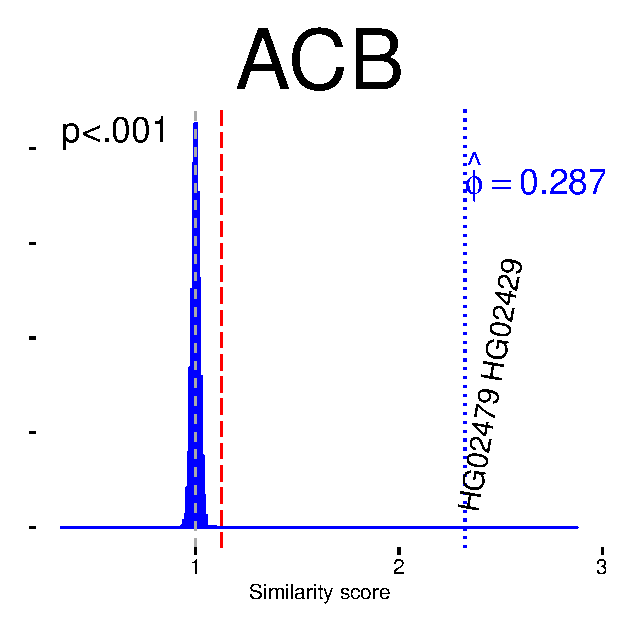
\includegraphics[width=0.12\paperwidth]{figures/PostFilter/ACBdiploid}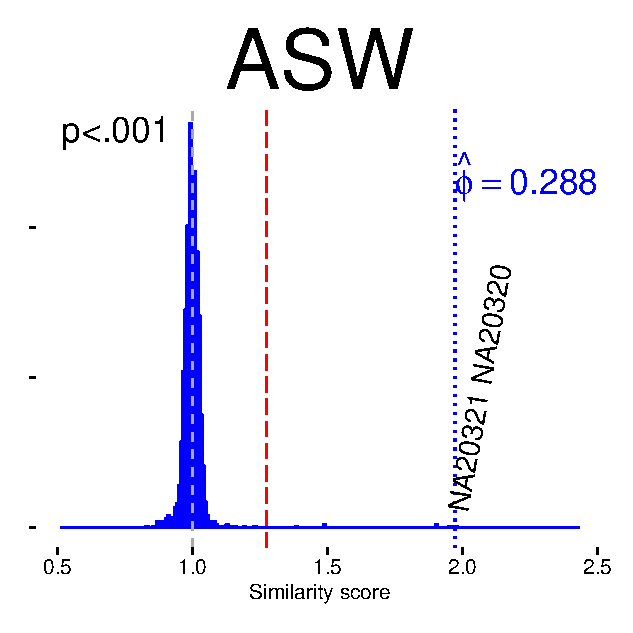
\includegraphics[width=0.12\paperwidth]{figures/PostFilter/ASWdiploid}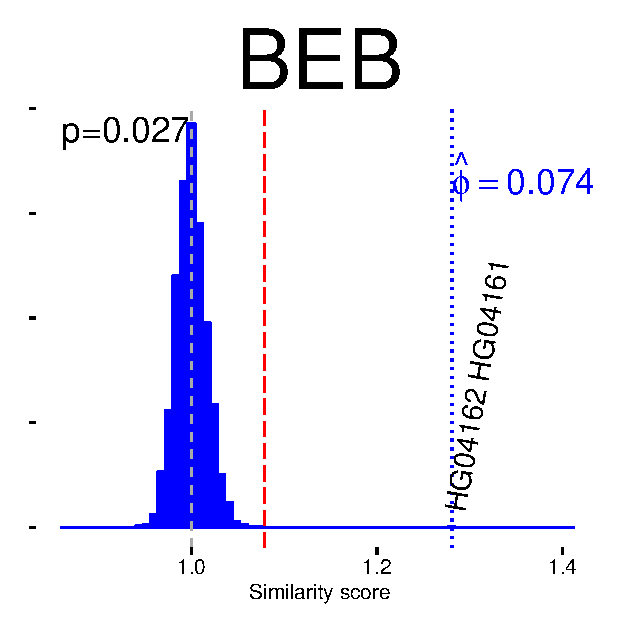
\includegraphics[width=0.12\paperwidth]{figures/PostFilter/BEBdiploid}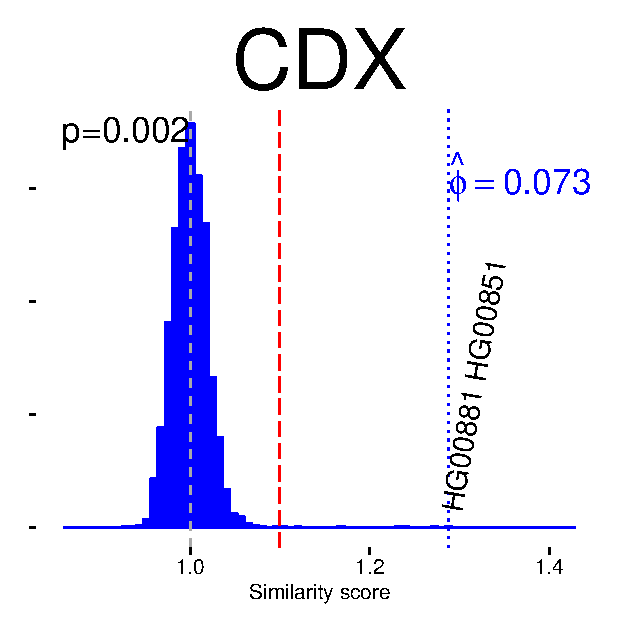
\includegraphics[width=0.12\paperwidth]{figures/PostFilter/CDXdiploid}\includegraphics[width=0.12\paperwidth]{figures/PostFilter/CEUdiploid}\includegraphics[width=0.12\paperwidth]{figures/PostFilter/CHBdiploid}

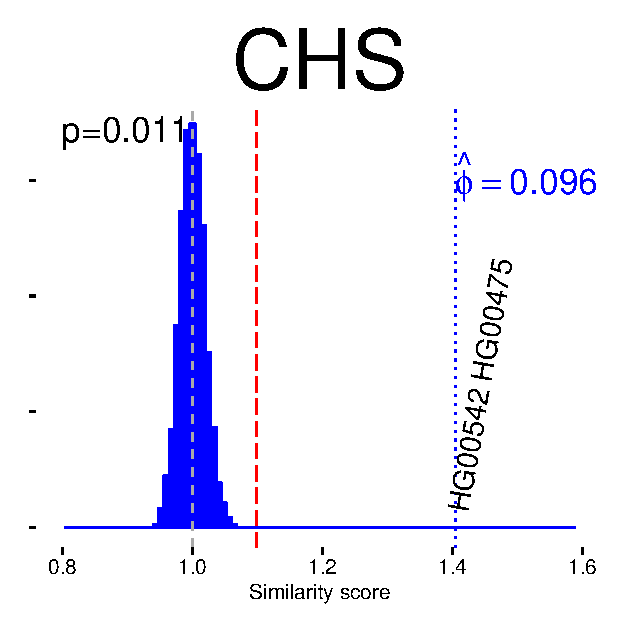
\includegraphics[width=0.12\paperwidth]{figures/PostFilter/CHSdiploid}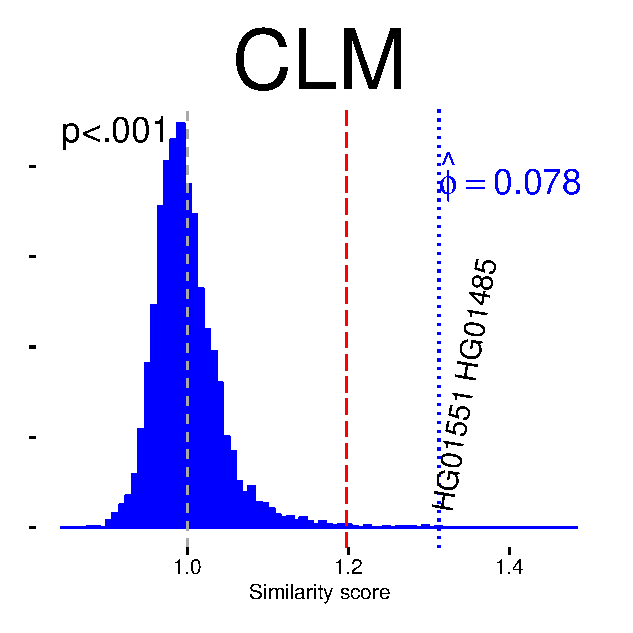
\includegraphics[width=0.12\paperwidth]{figures/PostFilter/CLMdiploid}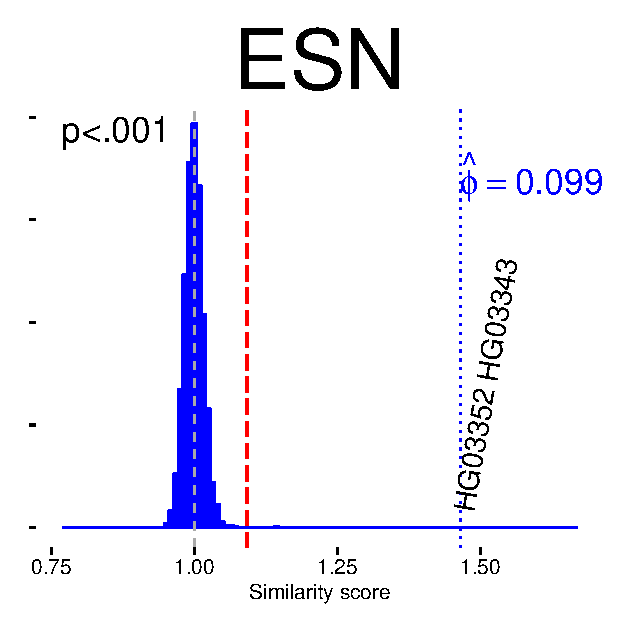
\includegraphics[width=0.12\paperwidth]{figures/PostFilter/ESNdiploid}\includegraphics[width=0.12\paperwidth]{figures/PostFilter/FINdiploid}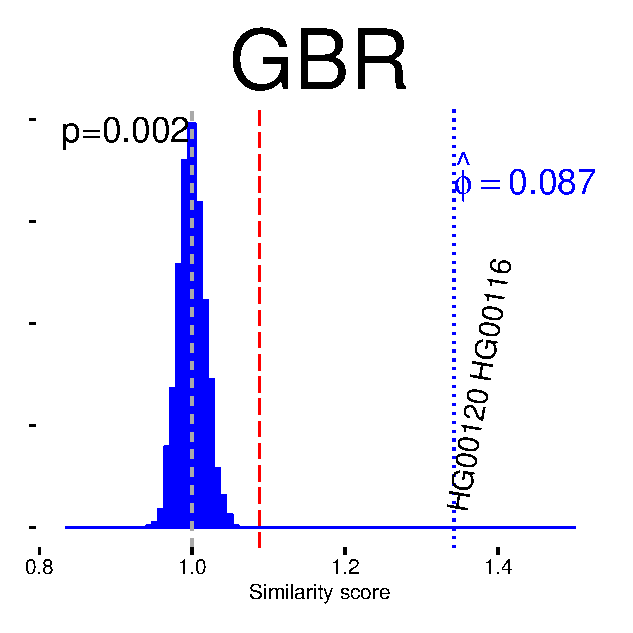
\includegraphics[width=0.12\paperwidth]{figures/PostFilter/GBRdiploid}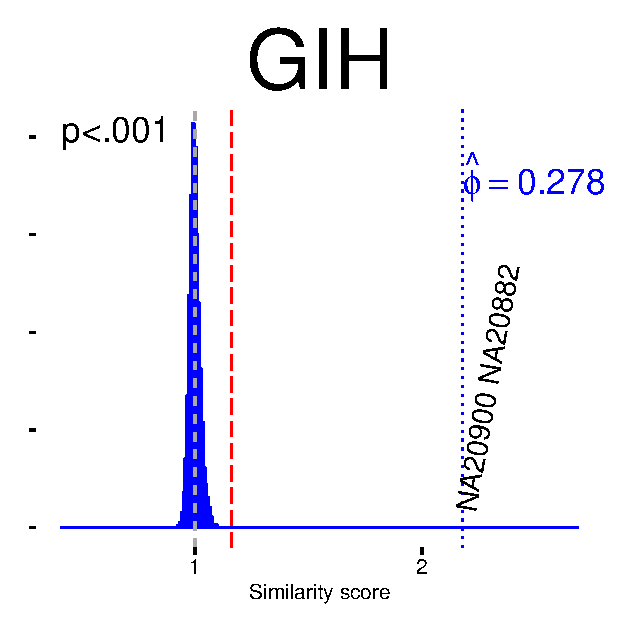
\includegraphics[width=0.12\paperwidth]{figures/PostFilter/GIHdiploid}

\includegraphics[width=0.12\paperwidth]{figures/PostFilter/GWDdiploid}\includegraphics[width=0.12\paperwidth]{figures/PostFilter/IBSdiploid}\includegraphics[width=0.12\paperwidth]{figures/PostFilter/ITUdiploid}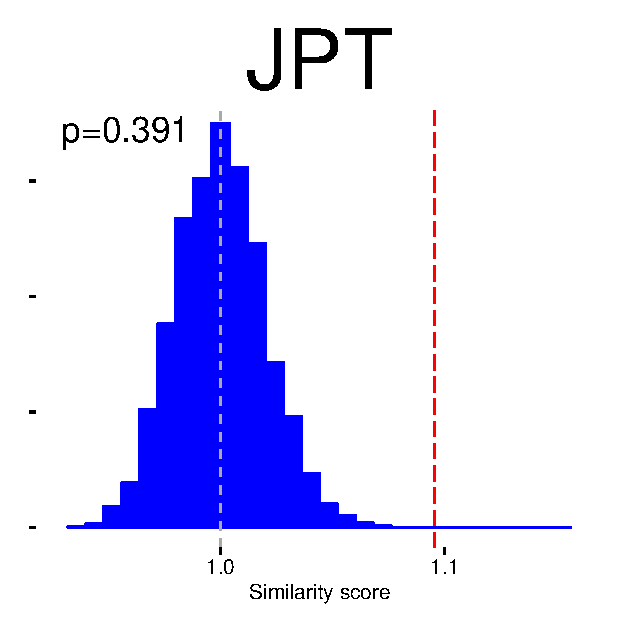
\includegraphics[width=0.12\paperwidth]{figures/PostFilter/JPTdiploid}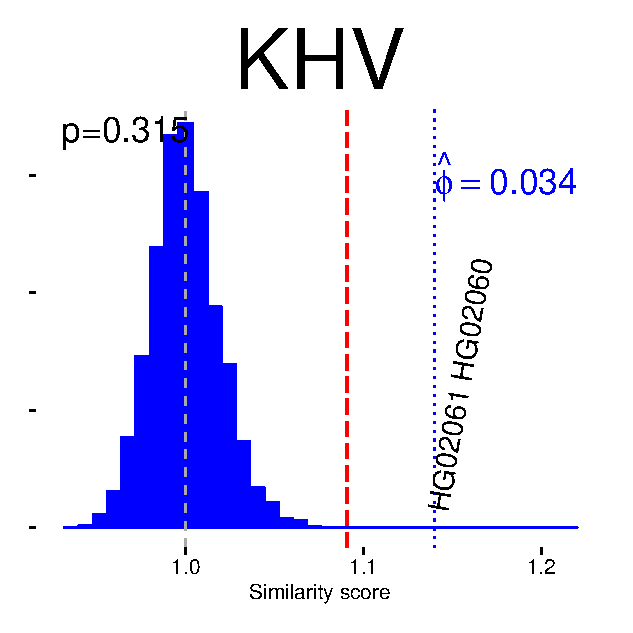
\includegraphics[width=0.12\paperwidth]{figures/PostFilter/KHVdiploid}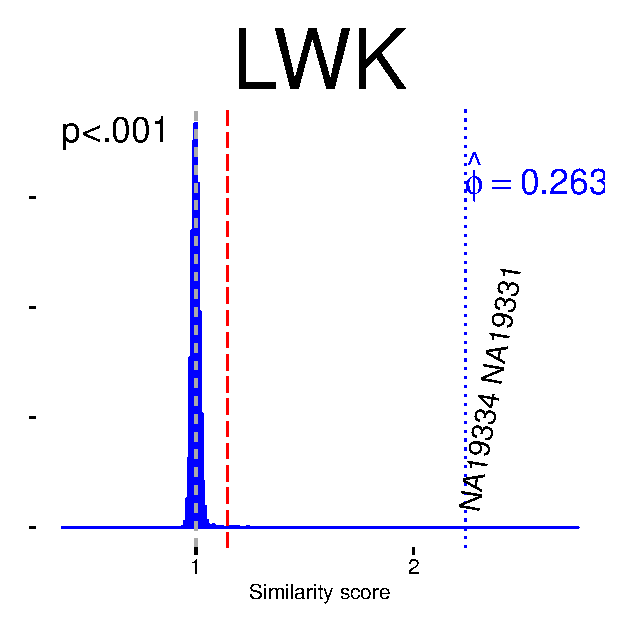
\includegraphics[width=0.12\paperwidth]{figures/PostFilter/LWKdiploid}

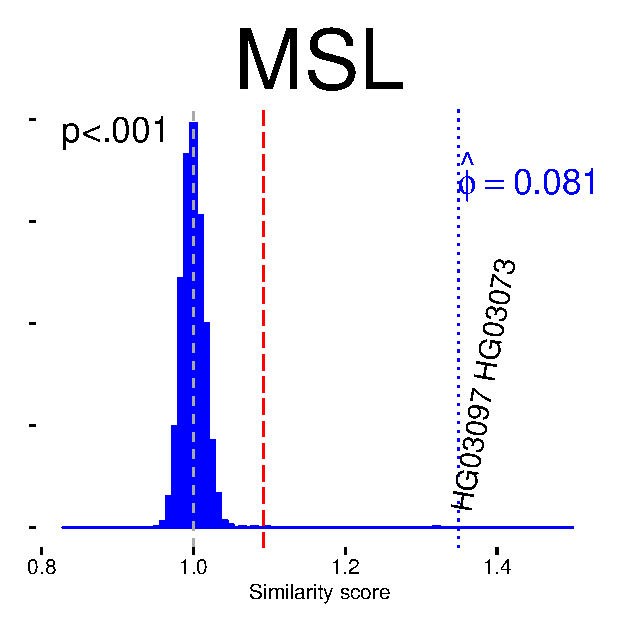
\includegraphics[width=0.12\paperwidth]{figures/PostFilter/MSLdiploid}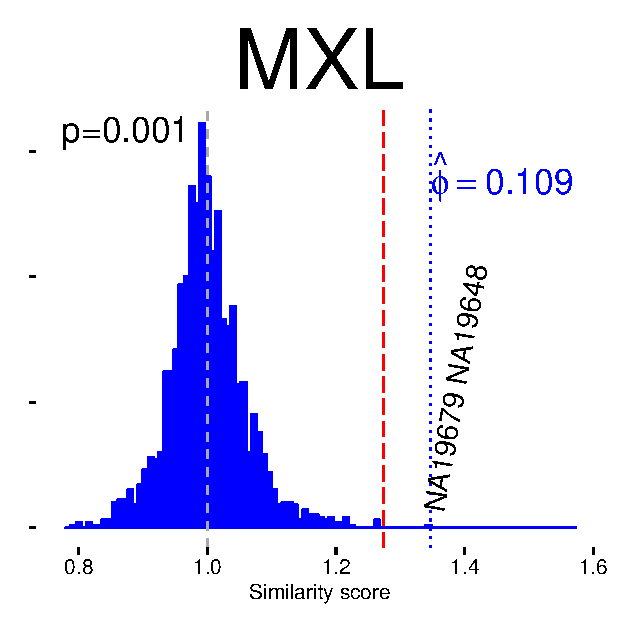
\includegraphics[width=0.12\paperwidth]{figures/PostFilter/MXLdiploid}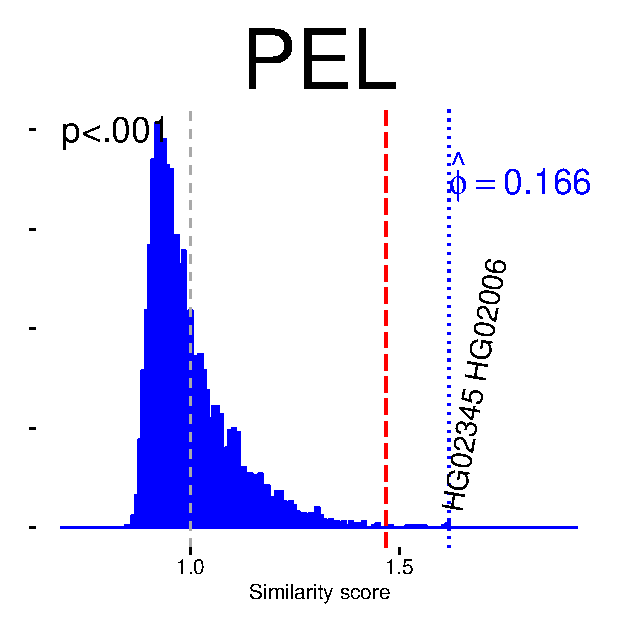
\includegraphics[width=0.12\paperwidth]{figures/PostFilter/PELdiploid}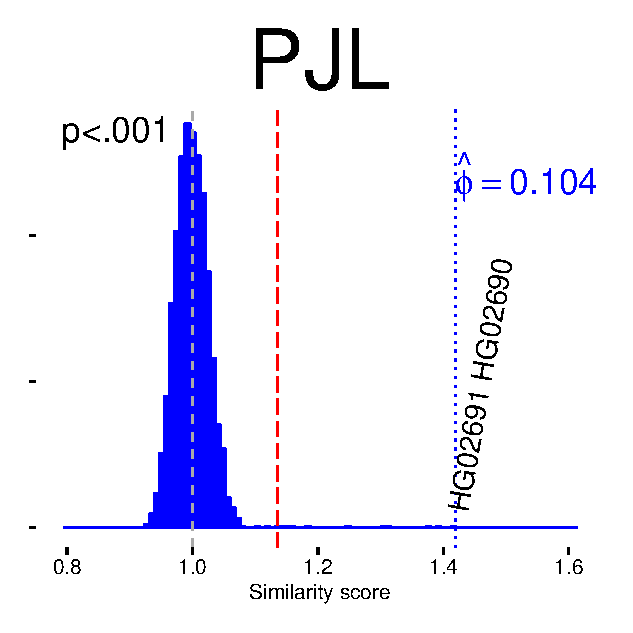
\includegraphics[width=0.12\paperwidth]{figures/PostFilter/PJLdiploid}\includegraphics[width=0.12\paperwidth]{figures/PostFilter/PURdiploid}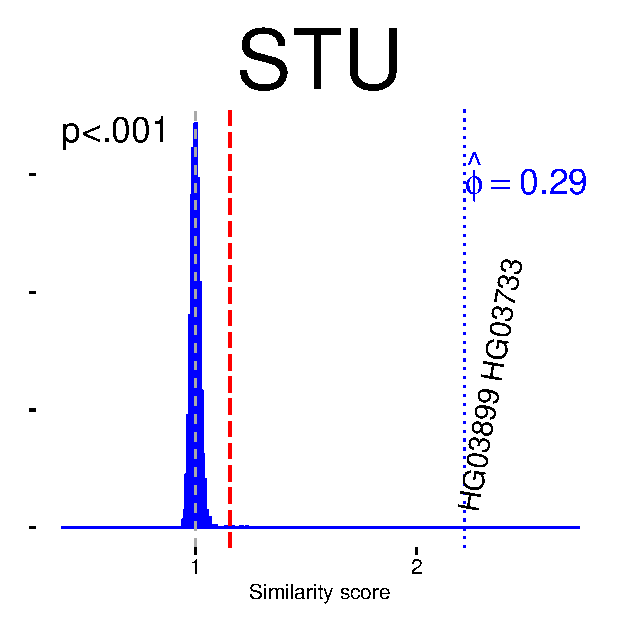
\includegraphics[width=0.12\paperwidth]{figures/PostFilter/STUdiploid}

\includegraphics[width=0.12\paperwidth]{figures/PostFilter/TSIdiploid}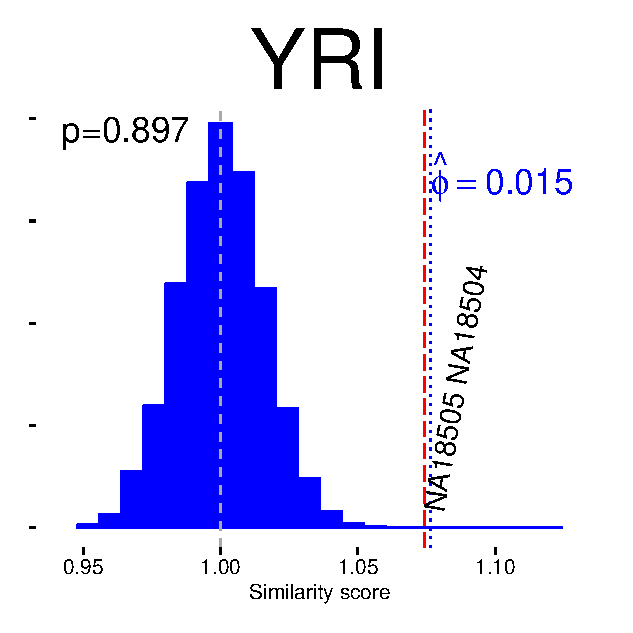
\includegraphics[width=0.12\paperwidth]{figures/PostFilter/YRIdiploid}\caption{Distribution of similarity coefficients for each of the 26 populations
in the 1000 Genomes Project after the removal of suspected related
individuals. Homogeneous populations lacking cryptic relatedness should
be expected to exhibit distributions centered around 1 with no outliers.
A heterogeneous population is expected to exhibit a normal distribution
centered around 1. Non-normal distributions such as right-skewed (e.g.
PUR, PEL, CLM) or bimodal are indicative of population structure.
The red dotted vertical line on each plot indicates the family-wise$\alpha=.01$
level cutoff for ${n \choose 2}$ comparisons. The most significant
related pair is labeled for each population with the estimated kinship
for that pairing indicated in blue. The p-value for the KS test for
homogeneity is reported for each population. Outliers in the absence
of non-normally distributed statistics are an indication of relatedness
among pairs of individuals.}
\label{All s plots-1}
\end{figure}

\begin{figure}
\textbf{A}\includegraphics[width=0.75\columnwidth]{figures/GSM_trim}

\textbf{B}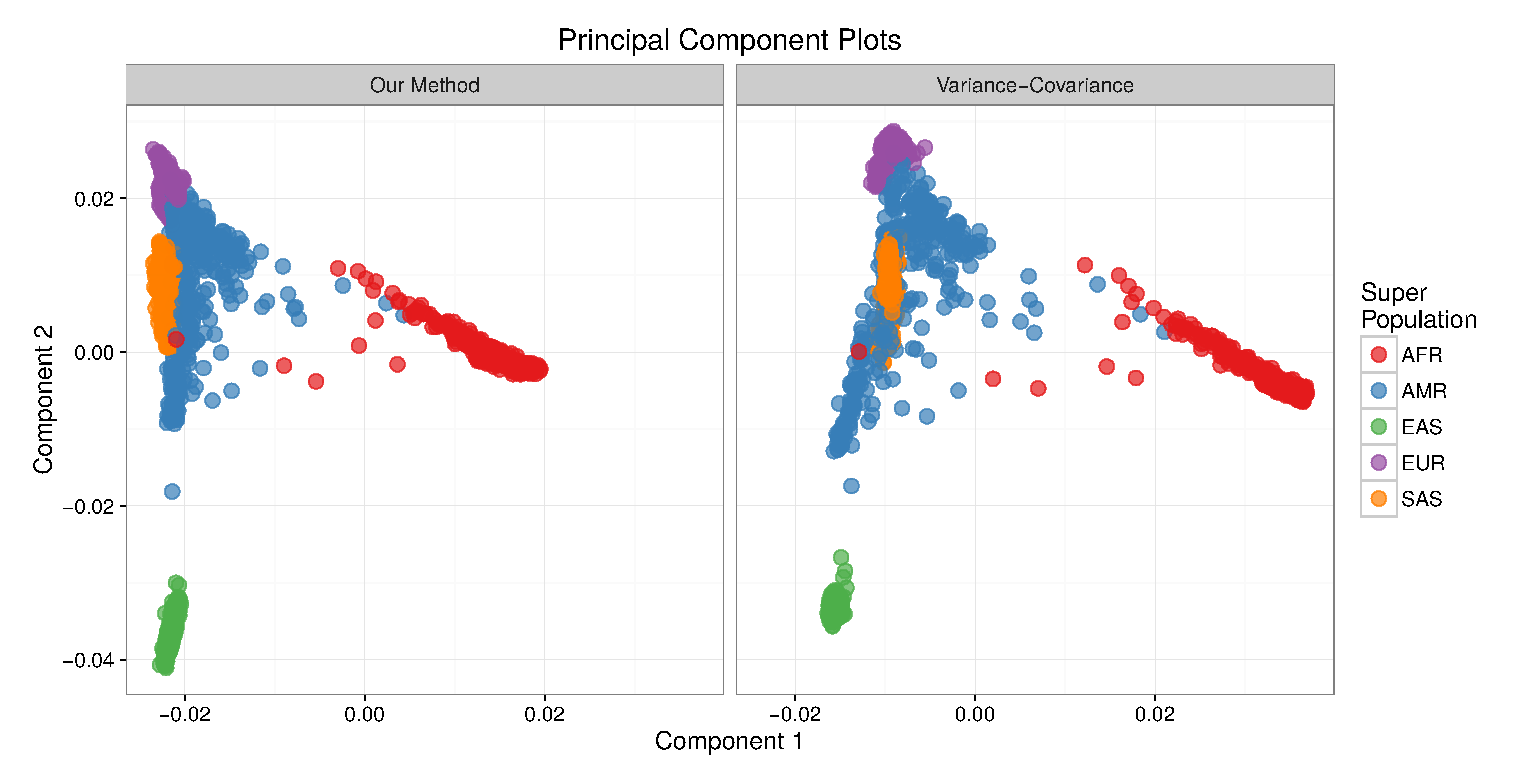
\includegraphics[width=0.8\columnwidth]{figures/PCA_all}\caption{Population structure in 2504 samples from 1000 Genomes Project. (\textbf{A})
Heatmap of the GSM generated by STEGO using 80,000 LD-sampled variants.
The vertical colorbar indicates membership in one of the five superpopulations,
while the horizontal colorbar indicates membership in one of the 26
populations. (\textbf{B}) Projecting each individual onto the top
two eigenvectors resulted in a similar 2-dimensional distribution
of global ancestry. Both STEGO and PCA show similar projections which
elucidate the migratory patterns of early humans.}
\label{fig: heatmaps}
\end{figure}
\begin{figure}
\includegraphics[width=1\columnwidth]{pasted2}\caption{Despite a clear trend of superior performance with STEGO, notable
exceptions occur. For example, by this measure, the populations GBR
and CEU were more clearly divided by PCA (Right) than by STEGO (Left).
Closer inspection revealed that the first eigenvector from STEGO isolates
11 samples exclusively from the GBR population. It is not readily
apparent what features of the data are being captured here or the
relative value of those features (this may be a result of population
structure, relatedness, batch effect, etc.). But it is notable that
all 11 samples came from the same population in the 1000 Genomes Project.
It is reasonable to infer that this subset of samples is scientifically
relevant. It most likely contains a disproportionate number of co-occurences
of rare variants, which were not observed separately by PCA.}
\end{figure}

\begin{figure}
 \resizebox{\columnwidth}{!}{%

\includegraphics{/home/dan/1000GP/supplemental_figure_wk}

}\caption{The weight factor, $w_{k}$, is shown here as a function of the minor
allele count in an example of 100 individuals (200 alleles) for each
locus, $k$. $w_{k}$ is monotonically decreasing for minor allele
counts greater than $1$, lending greater power to lower frequency
variants.  Typically, there will be a minimum minor allele count such
that the largest values for $w_{k}$are never obtained in practice}
\end{figure}

\begin{figure}
\includegraphics[width=1\columnwidth]{/home/dan/1000GP/plots/YRIvsAll_continent_color_interval}\label{YRIvsX}\caption{\textbf{Lower frequency alleles are more informative of ancestry.
}For the Yoruban population (YRI), this plot compares the average
unweighted Jaccard Index between individuals within group the to individuals
in all other populations of the 1000 Genomes Project. When filtering
by each minor allele frequency, we observe that low frequency alleles
create the strongest separation between populations. This trend holds
true for all but the lowest interval (0-0.4\% MAF), likely owing to
a tradeoff between rare variant informativeness and quality control
reliability.}
\end{figure}

\begin{figure}
\includegraphics[width=1\columnwidth]{/home/dan/1000GP/average_timing_comparison}\caption{\textbf{Average running time of STEGO is compared to the default implementations
of \textbf{cor()} and \textbf{princomp()} in R.} For each sample
size on the x-axis, 100,000 variants were randomly generated across
the samples. R functions for STEGO, correlation, and two implementations
of PCA (\textbf{prcomp }and \textbf{princomp}) were run 10 times on
each simulated dataset. Each of these methods has asymptotic computational
complexity of $\mathcal{O}(pN^{2})$, and we observe a consistent
speed improvement of approximately 3x for STEGO compared to \textbf{princomp()}.
This improvement scales linearly with increased number of variants,
which is most appealing for large whole genome sequencing studies
involving thousands of subjects and millions of variants.}
\label{comp_time}
\end{figure}

\begin{figure}
\includegraphics[width=0.6\columnwidth]{/home/dan/1000GP/simulated_PCP_plots}\caption{Principal Component plots for two methods for generating the genetic
similarity matrix. On the left, the GSM is generated via STEGO and
on the right the GSM uses the normalized covariance matrix. The STEGO
method makes more efficient use of the more ancestry informative rare
variants, providing a higher resolution separation of our two closely
related populations. Across the first two components the ratio of
within-population variance to total variance for STEGO vs variance-covariance
is .81 and .99, respectively.}
\label{simulatedPCP}
\end{figure}

\begin{figure}
\includegraphics[width=1\columnwidth]{figure1}\caption{The probability of rejecting the null hypothesis given a simulated
set of 301 homogeneous individuals containing a single related pair
with coefficient of kinship, $\phi$. The simulated power curve aligns
with the analytically derived expectation demonstrating the clearly
defined power of the method.}
\end{figure}

\begin{table}
\begin{tabular}{|c|c|c|c|}
\hline 
Population & Super Population & Structure & Cryptic Relatedness\tabularnewline
\hline 
\hline 
ACB & \multirow{7}{*}{AFR - African} & NO & NO\tabularnewline
\cline{1-1} \cline{3-4} 
ASW &  & NO & \textbf{YES}\tabularnewline
\cline{1-1} \cline{3-4} 
ESN &  & NO & NO\tabularnewline
\cline{1-1} \cline{3-4} 
GWD &  & NO & NO\tabularnewline
\cline{1-1} \cline{3-4} 
LWK &  & NO & NO\tabularnewline
\cline{1-1} \cline{3-4} 
MSL &  & NO & NO\tabularnewline
\cline{1-1} \cline{3-4} 
YRI &  & NO & YES\tabularnewline
\hline 
CLM & \multirow{4}{*}{AMR - Ad Mixed American} & \textbf{YES} & \textbf{YES}\tabularnewline
\cline{1-1} \cline{3-4} 
MXL &  & NO & NO\tabularnewline
\cline{1-1} \cline{3-4} 
PEL &  & \textbf{YES} & \textbf{YES}\tabularnewline
\cline{1-1} \cline{3-4} 
PUR &  & \textbf{YES} & \textbf{YES}\tabularnewline
\hline 
CDX & \multirow{5}{*}{EAS - East Asian} & NO & NO\tabularnewline
\cline{1-1} \cline{3-4} 
CHB &  & NO & NO\tabularnewline
\cline{1-1} \cline{3-4} 
CHS &  & NO & NO\tabularnewline
\cline{1-1} \cline{3-4} 
JPT &  & NO & NO\tabularnewline
\cline{1-1} \cline{3-4} 
KHV &  & NO & NO\tabularnewline
\hline 
CEU & \multirow{5}{*}{EUR - European} & NO & NO\tabularnewline
\cline{1-1} \cline{3-4} 
FIN &  & NO & NO\tabularnewline
\cline{1-1} \cline{3-4} 
GBR &  & NO & NO\tabularnewline
\cline{1-1} \cline{3-4} 
IBS &  & NO & NO\tabularnewline
\cline{1-1} \cline{3-4} 
TSI &  & NO & NO\tabularnewline
\hline 
BEB & \multirow{5}{*}{SAS - South Asian} & NO & NO\tabularnewline
\cline{1-1} \cline{3-4} 
GIH &  & \textbf{YES} & NO\tabularnewline
\cline{1-1} \cline{3-4} 
ITU &  & NO & NO\tabularnewline
\cline{1-1} \cline{3-4} 
PJL &  & NO & NO\tabularnewline
\cline{1-1} \cline{3-4} 
STU &  & NO & NO\tabularnewline
\hline 
\end{tabular}\caption{\textbf{Presence of population structure and cryptic relatedness detected
in each of the 26 populations in the 1000 Genomes Project.} STEGO
was run separately on each population group following the removal
of suspected related individuals. Population structure was defined
as a significant $\left(p<.01\right)$ Kolmogorov-Smirnov statistic
comparing the observed test statistic distribution to that expected
under the assumption of homogeneity. Cryptic relatedness was defined
as those populations containing at least one pair of individuals with
estimated kinship $\hat{\phi}>\frac{1}{32}$ and statistically significant
$\left(p<.01\right)$ kinship after multiple testing correction. }

\label{population_table}
\end{table}

\end{document}
